\documentclass[AutoFakeBold,AutoFakeSlant,scheme=plain,degree=bachelor,zihao=-4]{sustechthesis}

\usepackage[utf8]{inputenc} % allow utf-8 input
\usepackage[T1]{fontenc}    % use 8-bit T1 fonts
\usepackage{lmodern}        % https://github.com/rstudio/rticles/issues/343
\usepackage{hyperref}       % hyperlinks
\usepackage{url}            % simple URL typesetting
\usepackage{booktabs}       % professional-quality tables
\usepackage{amsfonts}       % blackboard math symbols
\usepackage{nicefrac}       % compact symbols for 1/2, etc.
\usepackage{microtype}      % microtypography
\usepackage{graphicx}

\title{SUSTech thesis R Markdown template}

\author{
  }


% tightlist command for lists without linebreak
\providecommand{\tightlist}{%
  \setlength{\itemsep}{0pt}\setlength{\parskip}{0pt}}

% From pandoc table feature
\usepackage{longtable,booktabs,array}
\usepackage{calc} % for calculating minipage widths
% Correct order of tables after \paragraph or \subparagraph
\usepackage{etoolbox}
\makeatletter
\patchcmd\longtable{\par}{\if@noskipsec\mbox{}\fi\par}{}{}
\makeatother
% Allow footnotes in longtable head/foot
\IfFileExists{footnotehyper.sty}{\usepackage{footnotehyper}}{\usepackage{footnote}}
\makesavenoteenv{longtable}

% Pandoc citation processing
\newlength{\cslhangindent}
\setlength{\cslhangindent}{1.5em}
\newlength{\csllabelwidth}
\setlength{\csllabelwidth}{3em}
\newlength{\cslentryspacingunit} % times entry-spacing
\setlength{\cslentryspacingunit}{\parskip}
% for Pandoc 2.8 to 2.10.1
\newenvironment{cslreferences}%
  {}%
  {\par}
% For Pandoc 2.11+
\newenvironment{CSLReferences}[2] % #1 hanging-ident, #2 entry spacing
 {% don't indent paragraphs
  \setlength{\parindent}{0pt}
  % turn on hanging indent if param 1 is 1
  \ifodd #1
  \let\oldpar\par
  \def\par{\hangindent=\cslhangindent\oldpar}
  \fi
  % set entry spacing
  \setlength{\parskip}{#2\cslentryspacingunit}
 }%
 {}
\usepackage{calc}
\newcommand{\CSLBlock}[1]{#1\hfill\break}
\newcommand{\CSLLeftMargin}[1]{\parbox[t]{\csllabelwidth}{#1}}
\newcommand{\CSLRightInline}[1]{\parbox[t]{\linewidth - \csllabelwidth}{#1}\break}
\newcommand{\CSLIndent}[1]{\hspace{\cslhangindent}#1}

% !Mode:: "TeX:UTF-8"
% !TEX program  = xelatex

% 数学符号与环境
\usepackage{amsmath,amssymb}
  \newcommand{\dd}{\mathrm{d}}
  \newcommand{\RR}{\mathbb{R}}
% 参考文献
\usepackage[style=gb7714-2015]{biblatex}
  \addbibresource{ref.bib}
% 无意义文本
\usepackage{zhlipsum,lipsum}
% 列表环境设置
\usepackage{enumitem}
% 浮动题不越过 \section
\usepackage[section]{placeins}
% 超链接
\usepackage{hyperref}
% 图片,子图,浮动题设置
\usepackage{graphicx,subcaption,float}
% 抄录环境设置,更多有趣例子请命令行输入 `texdoc tcolorbox`
\usepackage{tcolorbox}
  \tcbuselibrary{xparse}
  \DeclareTotalTCBox{\verbbox}{ O{green} v !O{} }%
    {fontupper=\ttfamily,nobeforeafter,tcbox raise base,%
    arc=0pt,outer arc=0pt,top=0pt,bottom=0pt,left=0mm,%
    right=0mm,leftrule=0pt,rightrule=0pt,toprule=0.3mm,%
    bottomrule=0.3mm,boxsep=0.5mm,bottomrule=0.3mm,boxsep=0.5mm,%
    colback=#1!10!white,colframe=#1!50!black,#3}{#2}%
\tcbuselibrary{listings,breakable}
  \newtcbinputlisting{\Python}[2]{
    listing options={language=Python,numbers=left,numberstyle=\tiny,
      breaklines,commentstyle=\color{white!50!black}\textit},
    title=\texttt{#1},listing only,breakable,
    left=6mm,right=6mm,top=2mm,bottom=2mm,listing file={#2}}
% 三线表支持
\usepackage{booktabs}

% LaTeX logo
\usepackage{hologo}
% !Mode:: "TeX:UTF-8"
% !TEX program  = xelatex
\设置信息{
    % 键 = {{中文值}, {英文值}},
    分类号 = {{}, {}},
    编号 = {{}, {}},
    UDC = {{}, {}},
    密级 = {{}, {}},
    % 仅题目(不含副标题)、系别、专业,支持手动 \\ 换行,不支持自动换行。
    题目 = {{南方科技大学毕业论文模板设计\\\hologo{LaTeX} 形式 v\version}, {Graduation Thesis Template\\\hologo{LaTeX} Format v\version}},
    % 如无需副标题,删除值内容即可,不可删除键定义。
    副标题 = {{副标题}, {Sub-title}},
    姓名 = {{梁钰栋}, {Iydon Liang}},
    学号 = {{11711217}, {11711217}},
    系别 = {{数学系}, {Department of Mathematics}},
    专业 = {{信息与计算科学}, {Computatoinal Mathematics}},
    指导老师 = {{高德纳}, {Donald~E.~Knuth}},
    时间 = {{2019年12月8日}, {December 8, 2019}},
    职称 = {{教授}, {Professor}},
}




\usepackage{amsthm}
\newtheorem{theorem}{Theorem}[section]
\newtheorem{lemma}{Lemma}[section]
\newtheorem{corollary}{Corollary}[section]
\newtheorem{proposition}{Proposition}[section]
\newtheorem{conjecture}{Conjecture}[section]
\theoremstyle{definition}
\newtheorem{definition}{Definition}[section]
\theoremstyle{definition}
\newtheorem{example}{Example}[section]
\theoremstyle{definition}
\newtheorem{exercise}{Exercise}[section]
\theoremstyle{definition}
\newtheorem{hypothesis}{Hypothesis}[section]
\theoremstyle{remark}
\newtheorem*{remark}{Remark}
\newtheorem*{solution}{Solution}
\begin{document}


\中文标题页\英文标题页
\中文诚信承诺书\英文诚信承诺书
\摘要标题
% % !Mode:: "TeX:UTF-8"
% !TEX program  = xelatex
\begin{中文摘要}{\LaTeX ;接口}
  笔者见到的毕业论文模板,大多是以文类的形式,少部分以宏包的形式,并且在模板中大多掺杂着各式各样的例子(除了维护频率高的模板),导致模板文件使用了大部分与形式格式不相关的内容,代码量巨大文档欠缺且不容易修改,出现问题需要查看宏包或者文类的源代码。于是,秉着仅提供实现最基本要求的理念,重构了之前所写的 \TeX\ 形式。由于第二年使用该模板,所以设计出的模板接口不能保证以后不发生重大变动,一切以文档为主。毕竟学校在发展初期,各类文件都在日渐完善,前几年时,学校标志及名称还发生变化,同时毕业论文的样式也发生了重大变化。但是可以保证的是,模板提供的接口均为中文形式\footnote{使用 \hologo{XeLaTeX} 特性,一方面增加辨识度,另一方面不拘泥于英文命名的规则。当然此举也有些许弊端,在此就不过多展开。},并且至少更新到 2021 年,也就是笔者毕业。模板这种东西不能保证一劳永逸,一方面学校的标准制度都在发生着改变,另一方面 \hologo{LaTeX} 的宏包也在发生着改变,早先流行的宏包可能几年后就被“淘汰”掉。因此,您的使用与反馈是我不断更新的动力,希望各位不吝赐教。
\end{中文摘要}

\begin{英文摘要}{LaTeX, Interface}
  \lipsum[1]
\end{英文摘要}
 % 论文摘要
\begin{中文摘要}{\LaTeX ;接口}
\lipsum[1]
\end{中文摘要}

\begin{英文摘要}{\LaTeX, R Markdown, pandoc}
\lipsum[1]
\end{英文摘要}

% \maketitle


% % \keywords{
%   %   \LaTeX, R Markdown, pandoc
%   % }
% 
\目录\clearpage % 目录及换页

Check \url{https://bookdown.org/yihui/bookdown/} and \url{https://bookdown.org/yihui/rmarkdown/} for detail introduction

\hypertarget{markdown-syntax}{%
\section{Markdown Syntax}\label{markdown-syntax}}

\textbf{EMTH}, \emph{Italic}, H\textsubscript{2}SO\textsubscript{4}, Fe\textsuperscript{2+}, Footnote\footnote{See \href{https://bookdown.org/yihui/bookdown/markdown-syntax.html}{markdown syntax}}

\begin{itemize}
\tightlist
\item
  list
\item
  list
\end{itemize}

\begin{enumerate}
\def\labelenumi{\arabic{enumi}.}
\tightlist
\item
  Numbered list
\item
  Numbered list
\end{enumerate}

\begin{enumerate}
\def\labelenumi{\alph{enumi}.}
\tightlist
\item
  Alternative numbered list
\item
  Alternative numbered list
\end{enumerate}

Inline Math \(a^2+b^2\), Math block:
\[
\sum_{i=1}^{\infty}\frac{1}{n^2}=\frac{\pi^2}{6}
\]

\hypertarget{markdown-extensions-by-bookdown}{%
\section{Markdown extensions by bookdown}\label{markdown-extensions-by-bookdown}}

Bookdown supply an extension of pandoc, which is already a superset of plain markdwon and TeX.

\hypertarget{cross-reference-and-citation}{%
\subsection{Cross reference and citation}\label{cross-reference-and-citation}}

Xie (\protect\hyperlink{ref-R-bookdown}{2020}) supply a neat way to do cross citation of ``theorems''(or numbered environment) and proofs(or unnumbered environment), in which you can write anything freely(even recursively)(\protect\hyperlink{ref-bookdown2016}{Xie 2016}; \protect\hyperlink{ref-rmarkdown2020}{Xie, Dervieux, and Riederer 2020}).

Check source code of theorem \ref{thm:t1}, figure \ref{fig:fig1}, table \ref{tab:tab1} to see how they work, then you will find two ways to cite(bracketed or not).

We refer to \href{https://bookdown.org/yihui/bookdown/markdown-extensions-by-bookdown.html\#theorems}{here} for the all supported environments.

\begin{theorem}[Fermat's Last Theorem]
\protect\hypertarget{thm:t1}{}\label{thm:t1}For \(n\ge 2\), there is no \(a,b,c\in \mathbb{N}^* \text{ s.t. }\)
\[
x^{n}+y^{n}=z^{n}
\]
\end{theorem}

\begin{proof}
I have discovered a truly marvelous proof of this, which this margin is too narrow to contain
\end{proof}

\begin{figure}

{\centering 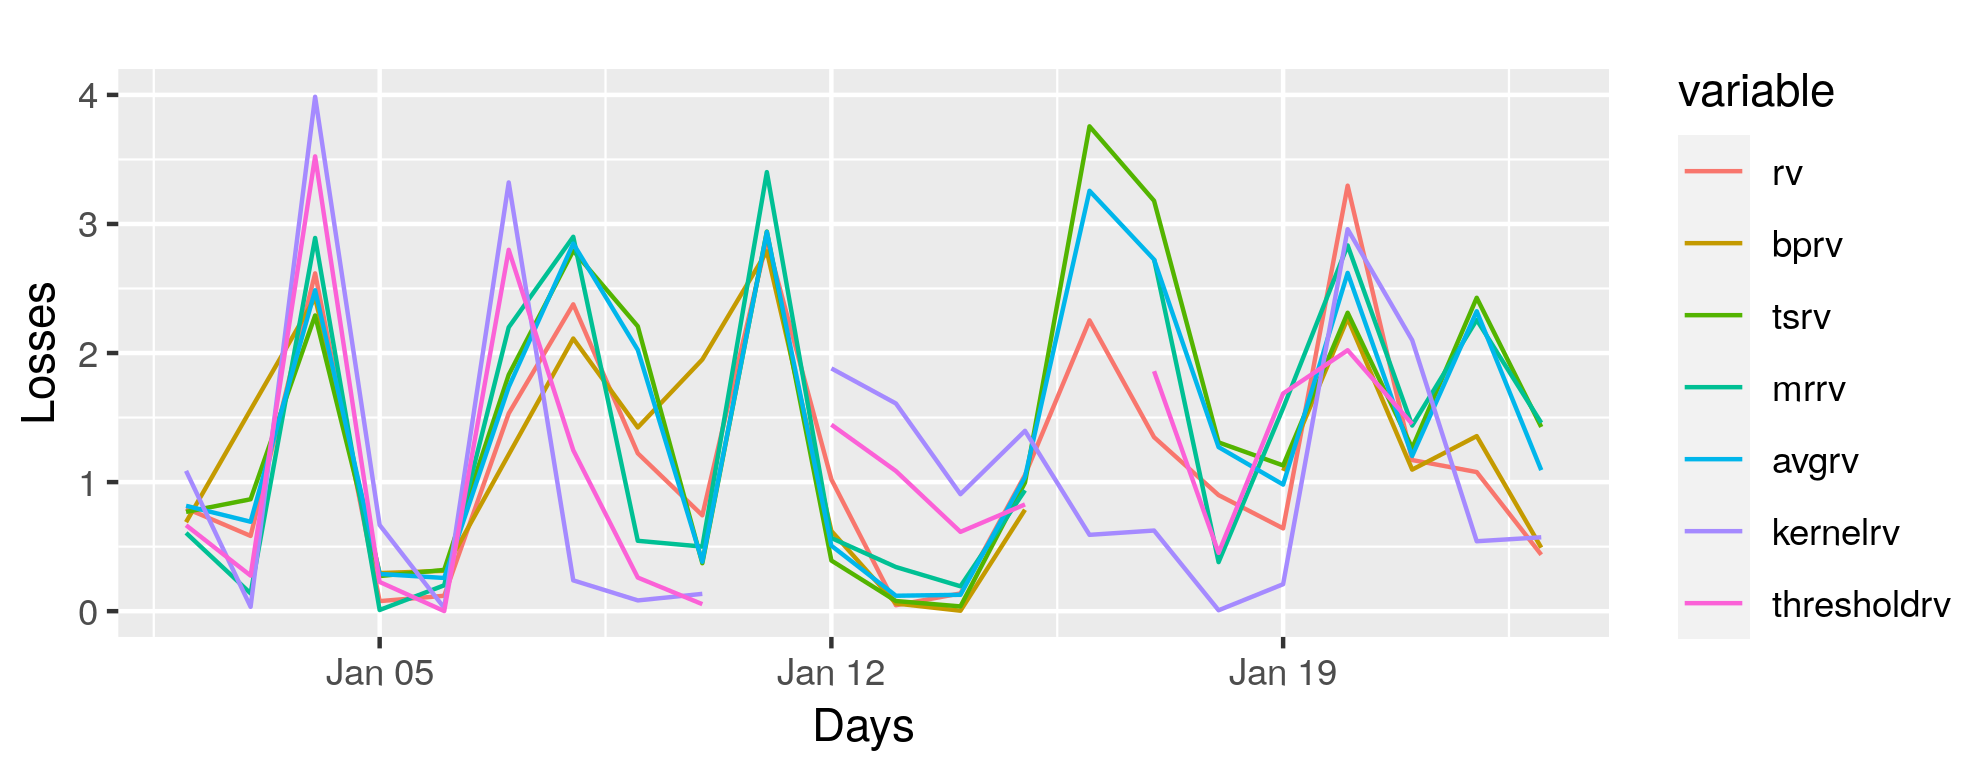
\includegraphics[width=0.7\linewidth]{figures/example-image-a} 

}

\caption{Text figures}\label{fig:fig1}
\end{figure}

\begin{table}

\caption{\label{tab:tab1}A table of the first 10 rows of the mtcars data.}
\centering
\begin{tabular}[t]{lrrrrrrrr}
\toprule
  & mpg & cyl & disp & hp & drat & wt & qsec & vs\\
\midrule
Mazda RX4 & 21.0 & 6 & 160.0 & 110 & 3.90 & 2.620 & 16.46 & 0\\
Mazda RX4 Wag & 21.0 & 6 & 160.0 & 110 & 3.90 & 2.875 & 17.02 & 0\\
Datsun 710 & 22.8 & 4 & 108.0 & 93 & 3.85 & 2.320 & 18.61 & 1\\
Hornet 4 Drive & 21.4 & 6 & 258.0 & 110 & 3.08 & 3.215 & 19.44 & 1\\
Hornet Sportabout & 18.7 & 8 & 360.0 & 175 & 3.15 & 3.440 & 17.02 & 0\\
\addlinespace
Valiant & 18.1 & 6 & 225.0 & 105 & 2.76 & 3.460 & 20.22 & 1\\
Duster 360 & 14.3 & 8 & 360.0 & 245 & 3.21 & 3.570 & 15.84 & 0\\
Merc 240D & 24.4 & 4 & 146.7 & 62 & 3.69 & 3.190 & 20.00 & 1\\
Merc 230 & 22.8 & 4 & 140.8 & 95 & 3.92 & 3.150 & 22.90 & 1\\
Merc 280 & 19.2 & 6 & 167.6 & 123 & 3.92 & 3.440 & 18.30 & 1\\
\bottomrule
\end{tabular}
\end{table}

\hypertarget{chapter}{%
\section{Chapter}\label{chapter}}

\lipsum[1]

\clearpage
\参考文献

\hypertarget{refs}{}
\begin{CSLReferences}{1}{0}
\leavevmode\vadjust pre{\hypertarget{ref-bookdown2016}{}}%
Xie, Yihui. 2016. \emph{Bookdown: Authoring Books and Technical Documents with {R} Markdown}. Boca Raton, Florida: Chapman; Hall/CRC. \url{https://github.com/rstudio/bookdown}.

\leavevmode\vadjust pre{\hypertarget{ref-R-bookdown}{}}%
---------. 2020. \emph{Bookdown: Authoring Books and Technical Documents with r Markdown}. \url{https://github.com/rstudio/bookdown}.

\leavevmode\vadjust pre{\hypertarget{ref-rmarkdown2020}{}}%
Xie, Yihui, Christophe Dervieux, and Emily Riederer. 2020. \emph{R Markdown Cookbook}. Boca Raton, Florida: Chapman; Hall/CRC. \url{https://bookdown.org/yihui/rmarkdown-cookbook}.

\end{CSLReferences}

\clearpage

\hypertarget{appendix}{%
\section*{Appendix}\label{appendix}}
\addcontentsline{toc}{section}{Appendix}

Attach code used here

\clearpage

\hypertarget{ux81f4ux8c22}{%
\section*{致谢}\label{ux81f4ux8c22}}
\addcontentsline{toc}{section}{致谢}

This repo credit to \href{}{rmarkdown}, \href{}{bookdown}, \href{}{knitr}.

% \bibliographystyle{unsrt}
% \bibliography{ref.bibpackages.bib}

% \参考文献
%   \printbibliography[heading=none]\clearpage


\end{document}
